\chapter{Implementation}
\label{ch:impl}

\section{Datasets}
\label{sec:datasets}
Three datasets were used (Table~\ref{tab:data}).

\minorhead{Travis~CI (development)}
The TravisTorrent export~\cite{beller2017travistorrent} contains 3.56 million job records. A Travis build runs several jobs, for example on different language versions. We collapsed the jobs into \textbf{858,368 builds} from \textbf{947 projects} (April~2011 to August~2016), checking that every pre-build field is identical across a build's jobs. A build fails if any of its jobs failed; 19.5\% of builds failed. A build's finish time is its start time plus its longest job's duration. Missing durations are filled with the repository's 95th-percentile duration.

\minorhead{GitHub Actions (external tests)}
On GitHub Actions the unit is a \emph{workflow run}. We kept first attempts of \texttt{push} and \texttt{pull\_request} runs. \texttt{success} is a pass, and \texttt{failure} and \texttt{startup\_failure} are failures; cancelled and skipped runs are excluded. A run's finish time is its \texttt{updated\_at}, and runs whose completion time is unknown are dropped. The size of each change (lines added and deleted, files changed, message length, parents) comes from the commits API.

The \emph{first} GitHub Actions dataset covers 30 repositories. The \emph{confirmation} dataset was collected with our own collector under a protocol fixed in advance. It takes the first 30 eligible repositories from a search of popular repositories, excluding all repositories used before, with runs created between 15~August and 30~September~2026. Of the qualifying runs, 3,773 (4.6\%) were dropped because their commits, mostly on deleted forks, could no longer be fetched.

\begin{table}[H]
\centering
\caption{Datasets used in the project}
\label{tab:data}
\begin{tabular}{|l|r|r|r|l|}
\hline
\textbf{Dataset} & \textbf{Builds / runs} & \textbf{Repos} & \textbf{Failure rate} & \textbf{Period}\\ \hline
Travis~CI (TravisTorrent) & 858,368 & 947 & 19.5\% & 2011--2016\\ \hline
GitHub Actions, test 1 & 67,980 & 30 & 8.9\% & 2025--2026\\ \hline
GitHub Actions, confirmation & 78,576 & 30 & 28.2\% & Aug--Sep 2026\\ \hline
GitHub Actions, combined & 146,556 & 60 & 19.2\% & 2025--2026\\ \hline
\end{tabular}
\end{table}

\section{Leakage-Safe Data Pipeline}
\label{sec:pipeline}
Most of the effort went into making sure that no model ever sees information it would not have when a build is triggered.

\minorhead{Availability registry}
Every column is recorded in a versioned registry with the stage at which it becomes known: pre-build, build start, or post-build. Fields computed from the build log, such as test counts, test duration and build duration, are marked post-build. So are comment counts, which can be written after the build. The predictor checks its inputs against the registry when it starts and refuses to run if any input is not available at prediction time.

\minorhead{Finish-time-safe history}
History features count a previous build only if it \emph{finished} strictly before the current build was triggered. Builds are processed per repository in time order, with a queue of builds still running; a build's outcome enters the history only once its finish time has passed. Ties are broken by finish time, then trigger time, then build id. In every evaluation run, a brute-force recomputation re-checks the history values on sampled repositories, and a deliberately leaked feature makes this check fail.

\minorhead{Finish buffers}
To test robustness, outcomes can be withheld for an extra 1 or 6 hours after a build finishes, which simulates delays in reporting.

\section{Feature Engineering}
\label{sec:features}
Features are organized in tiers (Table~\ref{tab:tiers}). A \emph{stream} is the build's pull request or, for push builds, its branch. On GitHub Actions, runs carry no pull request number, so a pull request is identified by its author and head branch.

{\renewcommand{\arraystretch}{1.3}
\begin{longtable}{|p{1.6cm}|p{12.2cm}|}
\caption{Feature tiers}\label{tab:tiers}\\
\hline
\textbf{Tier} & \textbf{Features}\\ \hline
\endfirsthead
\hline
\textbf{Tier} & \textbf{Features}\\ \hline
\endhead
Tier~A & \textbf{The change and its context} (18 features): source and test churn; files added, deleted and modified by type; hour, day, month, weekend and night flags; pull request flag; core-team author; default branch; and the project language. On GitHub Actions: lines added and deleted, files changed, message length, merge commit, default branch, and the workflow.\\ \hline
Tier~C & Tier~A plus \textbf{project context} (team size, code size, test density, past commits on the touched files, commits in the build) and \textbf{repository history}: the previous finished build's outcome and the repository's failure rate over the last 5 builds and overall.\\ \hline
Tier~E & Tier~C plus \textbf{stream history}: the outcome of the stream's last finished build; the stream's last-5 and overall failure rates, finished-build count and failure streak; the outcome of the build's predecessor (on Travis, the previous build on the branch; on GitHub Actions, the previous run of the same workflow on the stream); and an exponentially weighted repository failure rate.\newline
It also adds \textbf{in-flight context}: whether the previous build and the stream's last build are still running, how many builds are running in the repository, how many started in the last hour, and the hours since the stream last triggered. In-flight features use only the existence and start times of earlier builds, never their outcomes.\\ \hline
\end{longtable}}

\section{Prediction Models}
\label{sec:models}
\minorhead{Planned classifiers}
As planned, Random Forest, Decision Tree and SVM were trained, alongside XGBoost, LightGBM and a stacking ensemble (Random Forest, XGBoost and LightGBM combined by logistic regression). Hyperparameters were tuned with randomized search (25 settings, 3-fold cross-validation, F1 score) on a 200,000-row sample. The comparison is reported in Section~\ref{sec:leakage} as a \emph{development reference only}, because it uses a random split.

\minorhead{Final model: \tierE}
The final model combines two LightGBM models trained on \tierE\ features:
\begin{itemize}
\item a binary classifier, which predicts whether a build fails;
\item a ranker trained with the XE-NDCG objective~\cite{bruch2021alternative}, which learns to order builds within one repository and calendar month (one ranking ``query'').
\end{itemize}
Let $b(x)$ be the classifier's log-odds and $r(x)$ the ranker's score. Both are standardized with the mean and standard deviation of the \emph{training} scores and averaged:
\begin{equation}
s(x) = \tfrac{1}{2}\,\frac{r(x)-\mu_r}{\sigma_r} + \tfrac{1}{2}\,\frac{b(x)-\mu_b}{\sigma_b}.
\end{equation}
A Platt map~\cite{platt1999probabilistic} fitted on training scores turns $s(x)$ into a probability. LightGBM settings were fixed before any confirmation data was scored: 600 trees, learning rate 0.03, 63 leaves, at least 200 samples per leaf, 80\% row and column sampling, and L2 regularization 1.0.

\minorhead{Deployed model}
The deployed model is trained on walk-forward folds 1--9 of the 146,556 GitHub Actions runs, with the newest 10\% held out. Before it is saved, it must reproduce the research evaluation's predictions on the held-out fold; the largest difference was 0. Explanations use SHAP values of the binary half of the model.

\section{Anomaly, Bottleneck and Root Cause Modules}
\label{sec:aux}
\begin{itemize}
\item \textbf{Bottleneck detection.} For every completed GitHub Actions job, the system compares its duration with at least 10 earlier runs of the same job. A job that exceeds both their 95th percentile and the median plus three median absolute deviations is marked as a bottleneck. A scheduled collector also checks jobs that are still running, so stalled jobs are flagged while they run.
\item \textbf{Anomaly detection.} An Isolation Forest (10\% contamination) flags builds whose pre-build input profile is unusual. Because such builds did not fail more often, the flag is kept as a diagnostic and not shown as a failure prediction.
\item \textbf{Root cause analysis.} Failed-test text is clustered with TF-IDF and k-means. Failed GitHub Actions job logs, uploaded by an optional workflow, are sanitized and diagnosed with ordered rules into five categories. Each category maps to a suggestion, for example retrying transient tests and mocking external calls, or pinning compatible dependency versions.
\end{itemize}

\section{Deployed System}
\label{sec:deployed}
\begin{figure}[H]
\centering
\begin{tikzpicture}[
  font=\small,
  box/.style={draw, rounded corners=3pt, align=center, minimum height=11mm, text width=32mm, inner sep=2pt, fill=white},
  arr/.style={-{Stealth[length=2.2mm]}, thick},
  lab/.style={font=\footnotesize, fill=white, inner sep=1pt}]
\node[box, fill=blue!7] (gh) at (0,0) {GitHub Actions};
\node[box] (hook) at (5,0) {Webhook\\(signature check)};
\node[box] (ctx) at (10,0) {Stream \& in-flight\\context (database)};
\node[box, fill=green!7] (db) at (0,-2.6) {Builds \&\\predictions};
\node[box] (alert) at (5,-2.6) {Per-repository\\alert budget};
\node[box, fill=violet!7] (model) at (10,-2.6) {\tierE\ model\\+ SHAP};
\node[box, fill=green!7] (ui) at (0,-5.2) {Dashboard};
\node[box, fill=blue!7] (cmt) at (10,-5.2) {Commits API\\(change size)};
\draw[arr] (gh) -- node[lab, above=3pt] {requested} (hook);
\draw[arr] (hook) -- (ctx);
\draw[arr] (ctx) -- (model);
\draw[arr] (model) -- (alert);
\draw[arr] (alert) -- (db);
\draw[arr] (db) -- (ui);
\draw[arr] (cmt) -- (model);
\draw[arr, dashed] (gh) -- node[lab, left=1pt] {completed} (db);
\draw[arr, dotted] (db.north east) -- node[lab] {history} (ctx.south west);
\end{tikzpicture}
\caption{Scoring path of the deployed system}
\label{fig:scoring}
\end{figure}

\minorhead{Scoring path}
Fig~\ref{fig:scoring} shows the scoring path. A FastAPI service receives signed GitHub \texttt{workflow\_run} events.
\begin{enumerate}
\item When a run is \emph{requested}, before it executes, the service builds the run's stream history and in-flight context from the repository's stored runs, and fetches the commit's size from the GitHub API.
\item It scores the run with \tierE\ and stores a shadow prediction with its explanation.
\item When the run \emph{completes}, its real outcome is attached and becomes history for later runs. Other conclusions, such as cancelled runs, are stored but never become history, as in training.
\end{enumerate}
Runs are timed by GitHub's own creation and completion times, so a late webhook delivery cannot change a run's history. The system is advisory and never blocks CI.

\minorhead{Same history live as in training}
Automated tests replay synthetic run histories through both the offline training pass and the live service, and check that every history and in-flight value matches, row by row.

\minorhead{Per-repository alert budget}
A single global threshold flags too many runs in risky repositories and almost none in safe ones. Instead, a run becomes an alert when its risk reaches the 85th percentile of its \emph{own repository's} last 100 scored runs: each repository reviews its riskiest 15\%. Until a repository has 20 scored runs, a ``typical repository'' threshold of 0.893 is used. Neither threshold uses outcome labels. Section~\ref{sec:alerts} evaluates this policy.

\minorhead{Public demonstration}
A read-only demonstration runs on Render as a single Docker container that serves the dashboard and the API from one address. It replays 450 real GitHub Actions runs from \texttt{twbs/bootstrap}, \texttt{freeCodeCamp} and \texttt{yt-dlp} through the real webhook, at their real times. The runs come from the model's held-out period, so every prediction shown is out-of-sample, and contributor and branch names are replaced with pseudonyms. Visitors can explore every page and score builds, but nothing is saved.

\section{Dashboard}
\label{sec:dashboard}
The dashboard has four pages.

\minorhead{Dashboard}
Summary cards, the daily trend of average predicted risk against the actual failure rate (Fig~\ref{fig:dash_overview}), the distribution of predicted risk, and a model-evidence panel with the research results (Fig~\ref{fig:dash_models}, Chapter~\ref{ch:results}).

\begin{figure}[H]
\centering
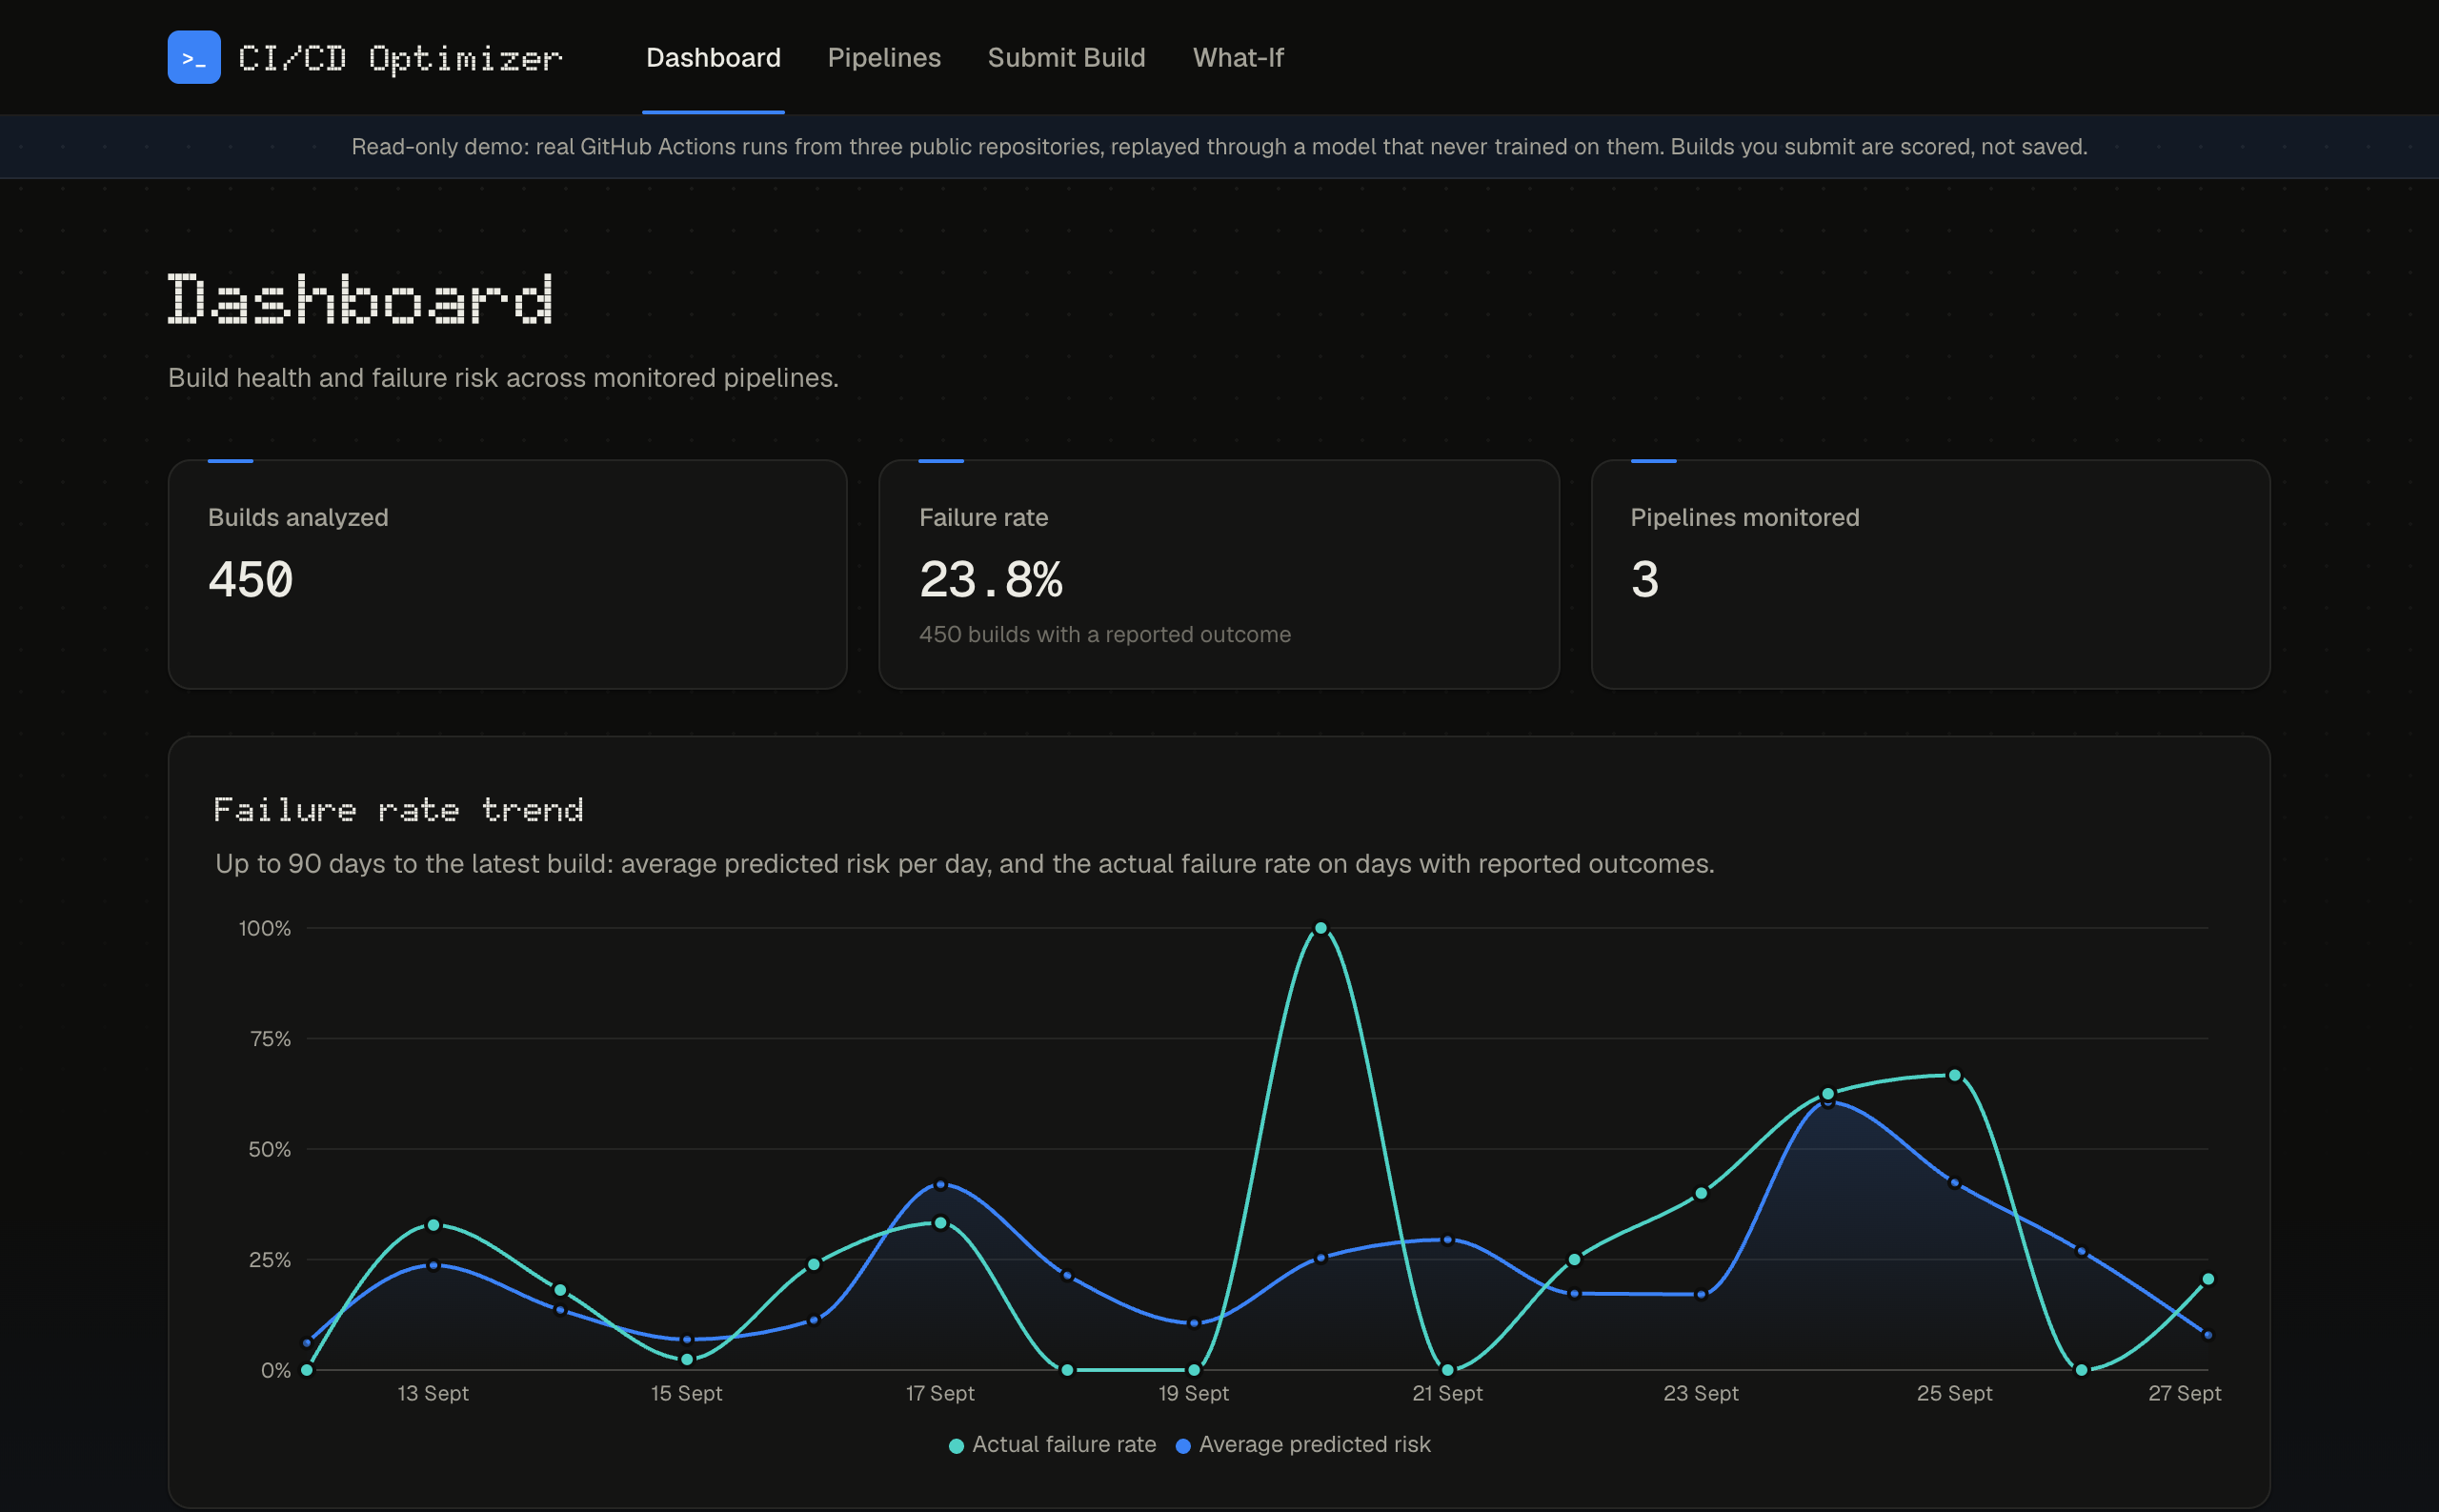
\includegraphics[width=0.92\textwidth]{dashboard_overview.png}
\caption{Dashboard: summary cards and daily failure-rate trend (public demonstration)}
\label{fig:dash_overview}
\end{figure}

\minorhead{Pipelines}
Each repository's latest status and risk, with a sparkline of its recent risk (Fig~\ref{fig:pipelines}). A repository's page shows its risk over time, with each run colored by its real outcome and the repository's alert threshold as a dashed line (Fig~\ref{fig:timeline}). It also lists every build with its explanation and a downloadable PDF report.

\begin{figure}[H]
\centering
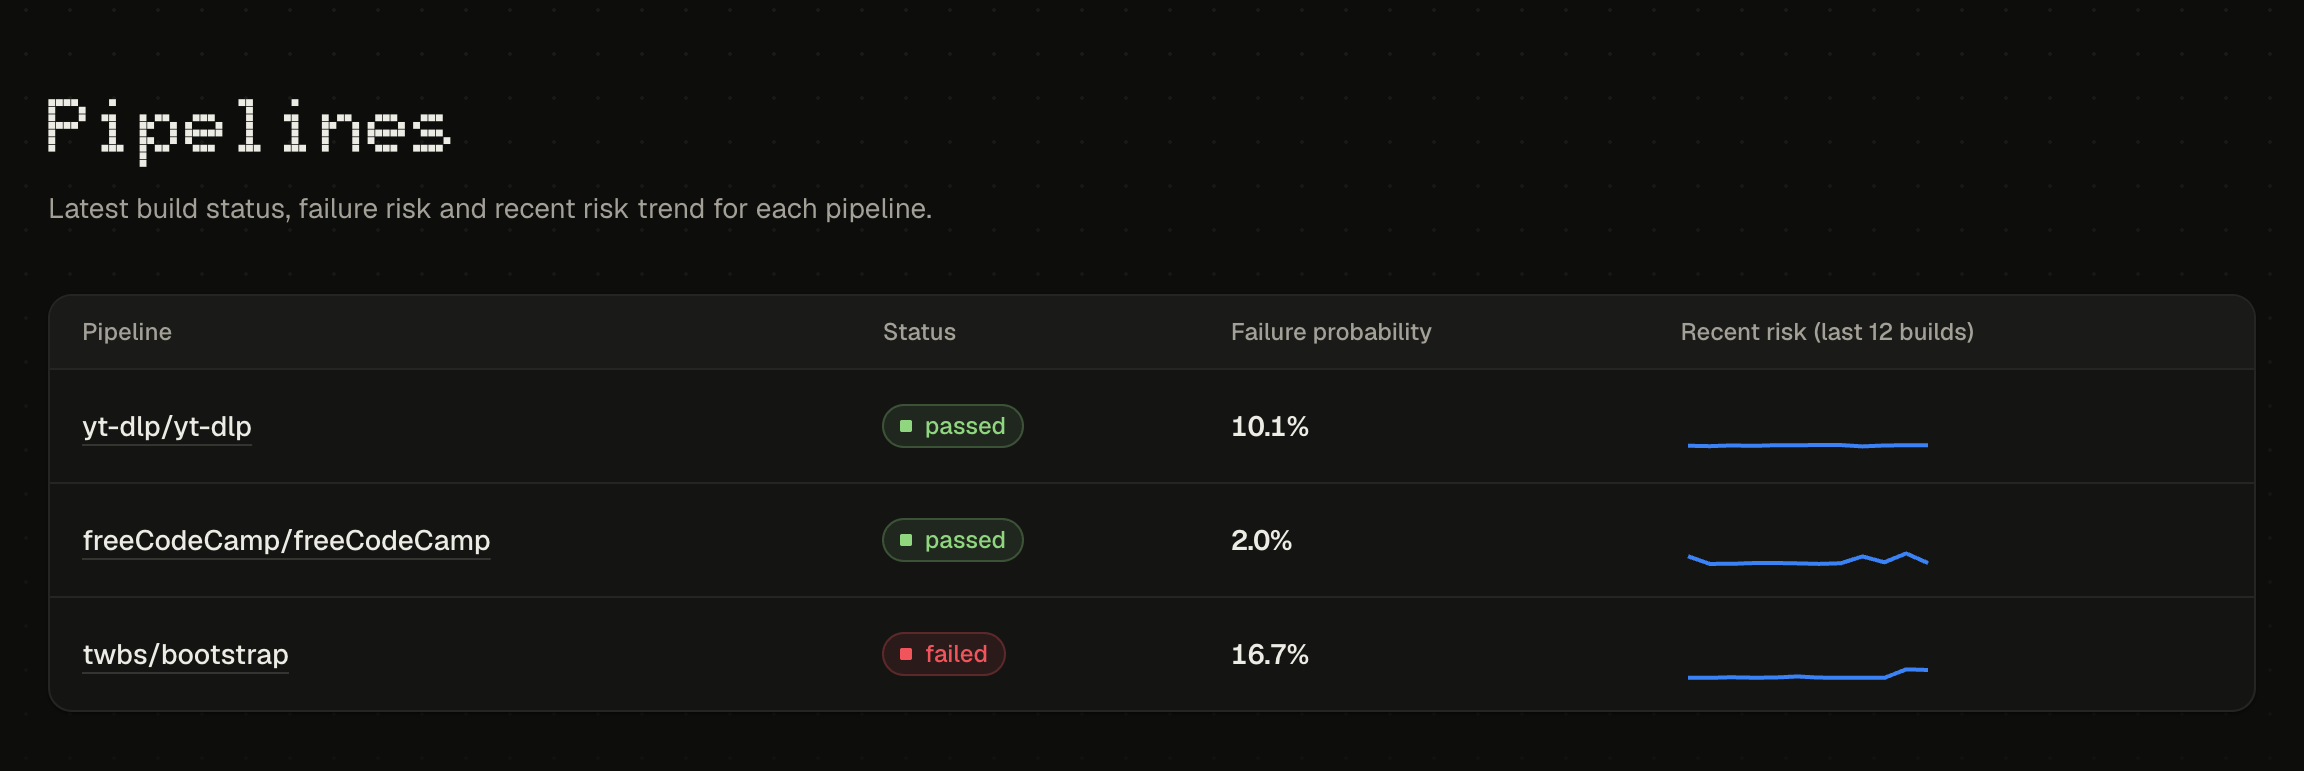
\includegraphics[width=0.92\textwidth]{pipelines.png}
\caption{Pipelines page with recent-risk sparklines}
\label{fig:pipelines}
\end{figure}

\begin{figure}[H]
\centering
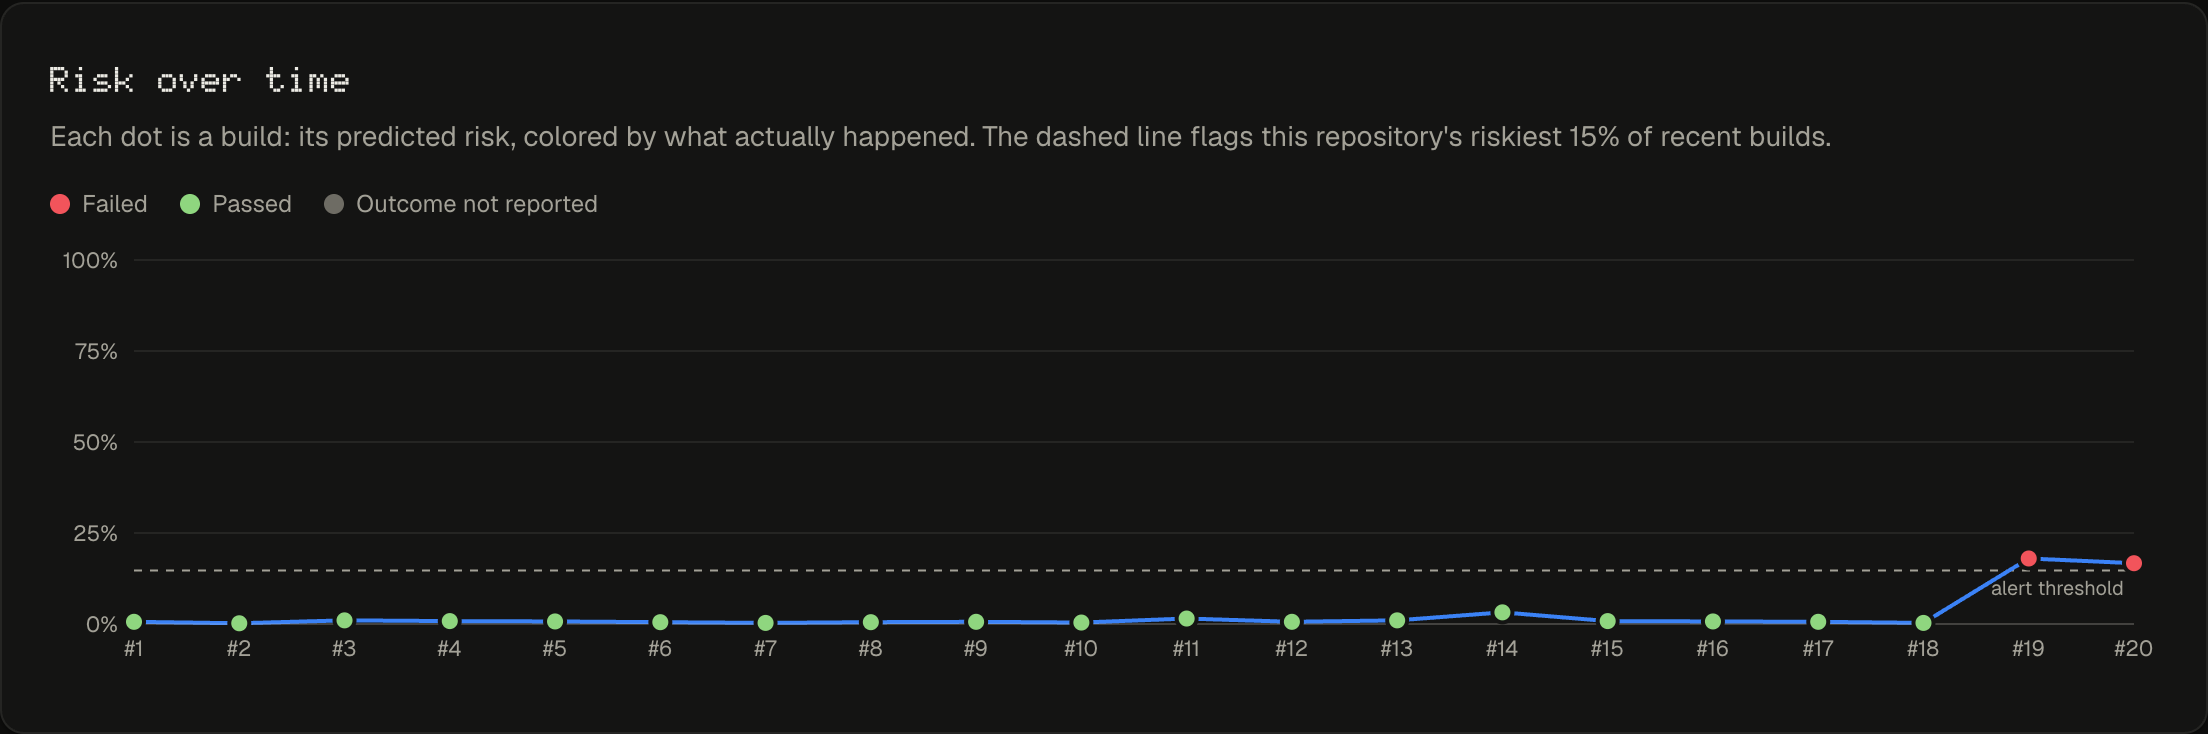
\includegraphics[width=\textwidth]{pipeline_timeline.png}
\caption{Risk timeline of \texttt{twbs/bootstrap}. The two newest runs, both real failures, rise above the repository's alert threshold.}
\label{fig:timeline}
\end{figure}

\minorhead{Submit Build}
Scores a GitHub Actions run described by its repository, workflow, pull request author and branch, and commit size. It shows the history the server derived for it and compares the risk with the repository's own threshold (Fig~\ref{fig:submit}).

\begin{figure}[H]
\centering
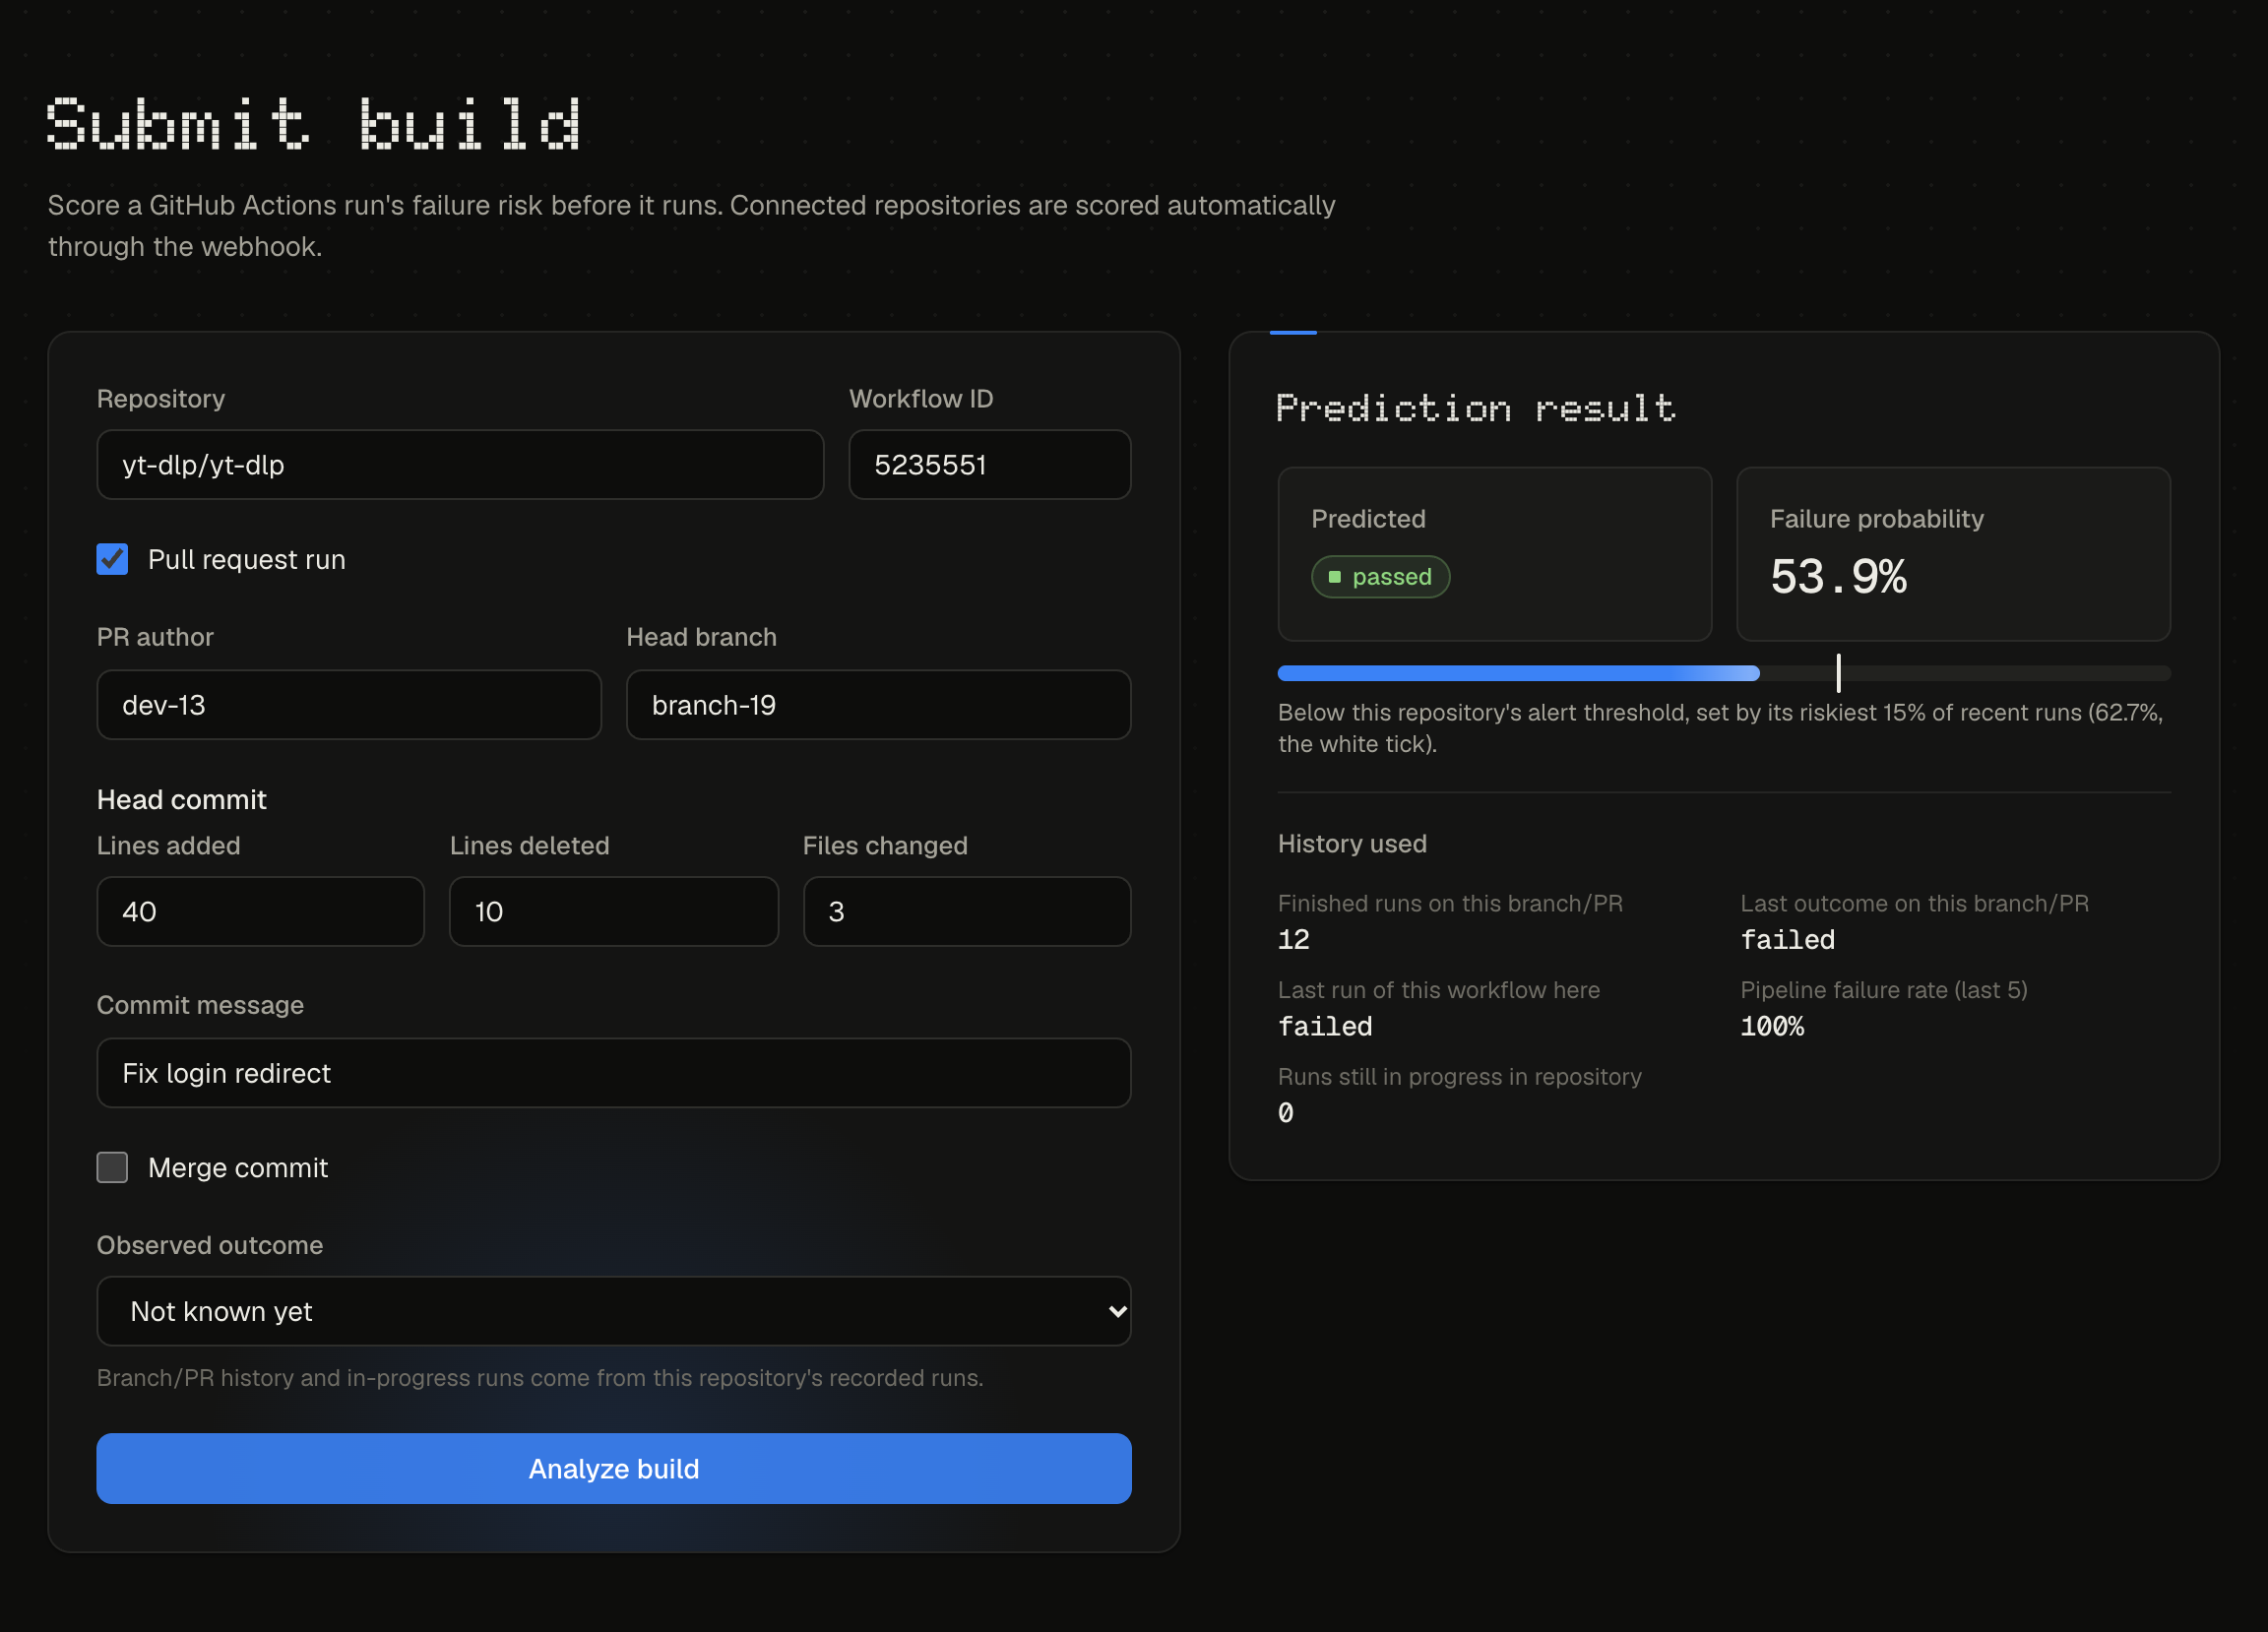
\includegraphics[width=0.9\textwidth]{submit_result.png}
\caption{Submit Build: a run on a failing \texttt{yt-dlp} branch, scored with server-derived history}
\label{fig:submit}
\end{figure}

\minorhead{What-If}
Changes inputs and immediately shows how the risk moves, with SHAP explanations and a trail of the risk across edits (Fig~\ref{fig:whatif}). An optimization simulation compares one changed input against the baseline.

\begin{figure}[H]
\centering
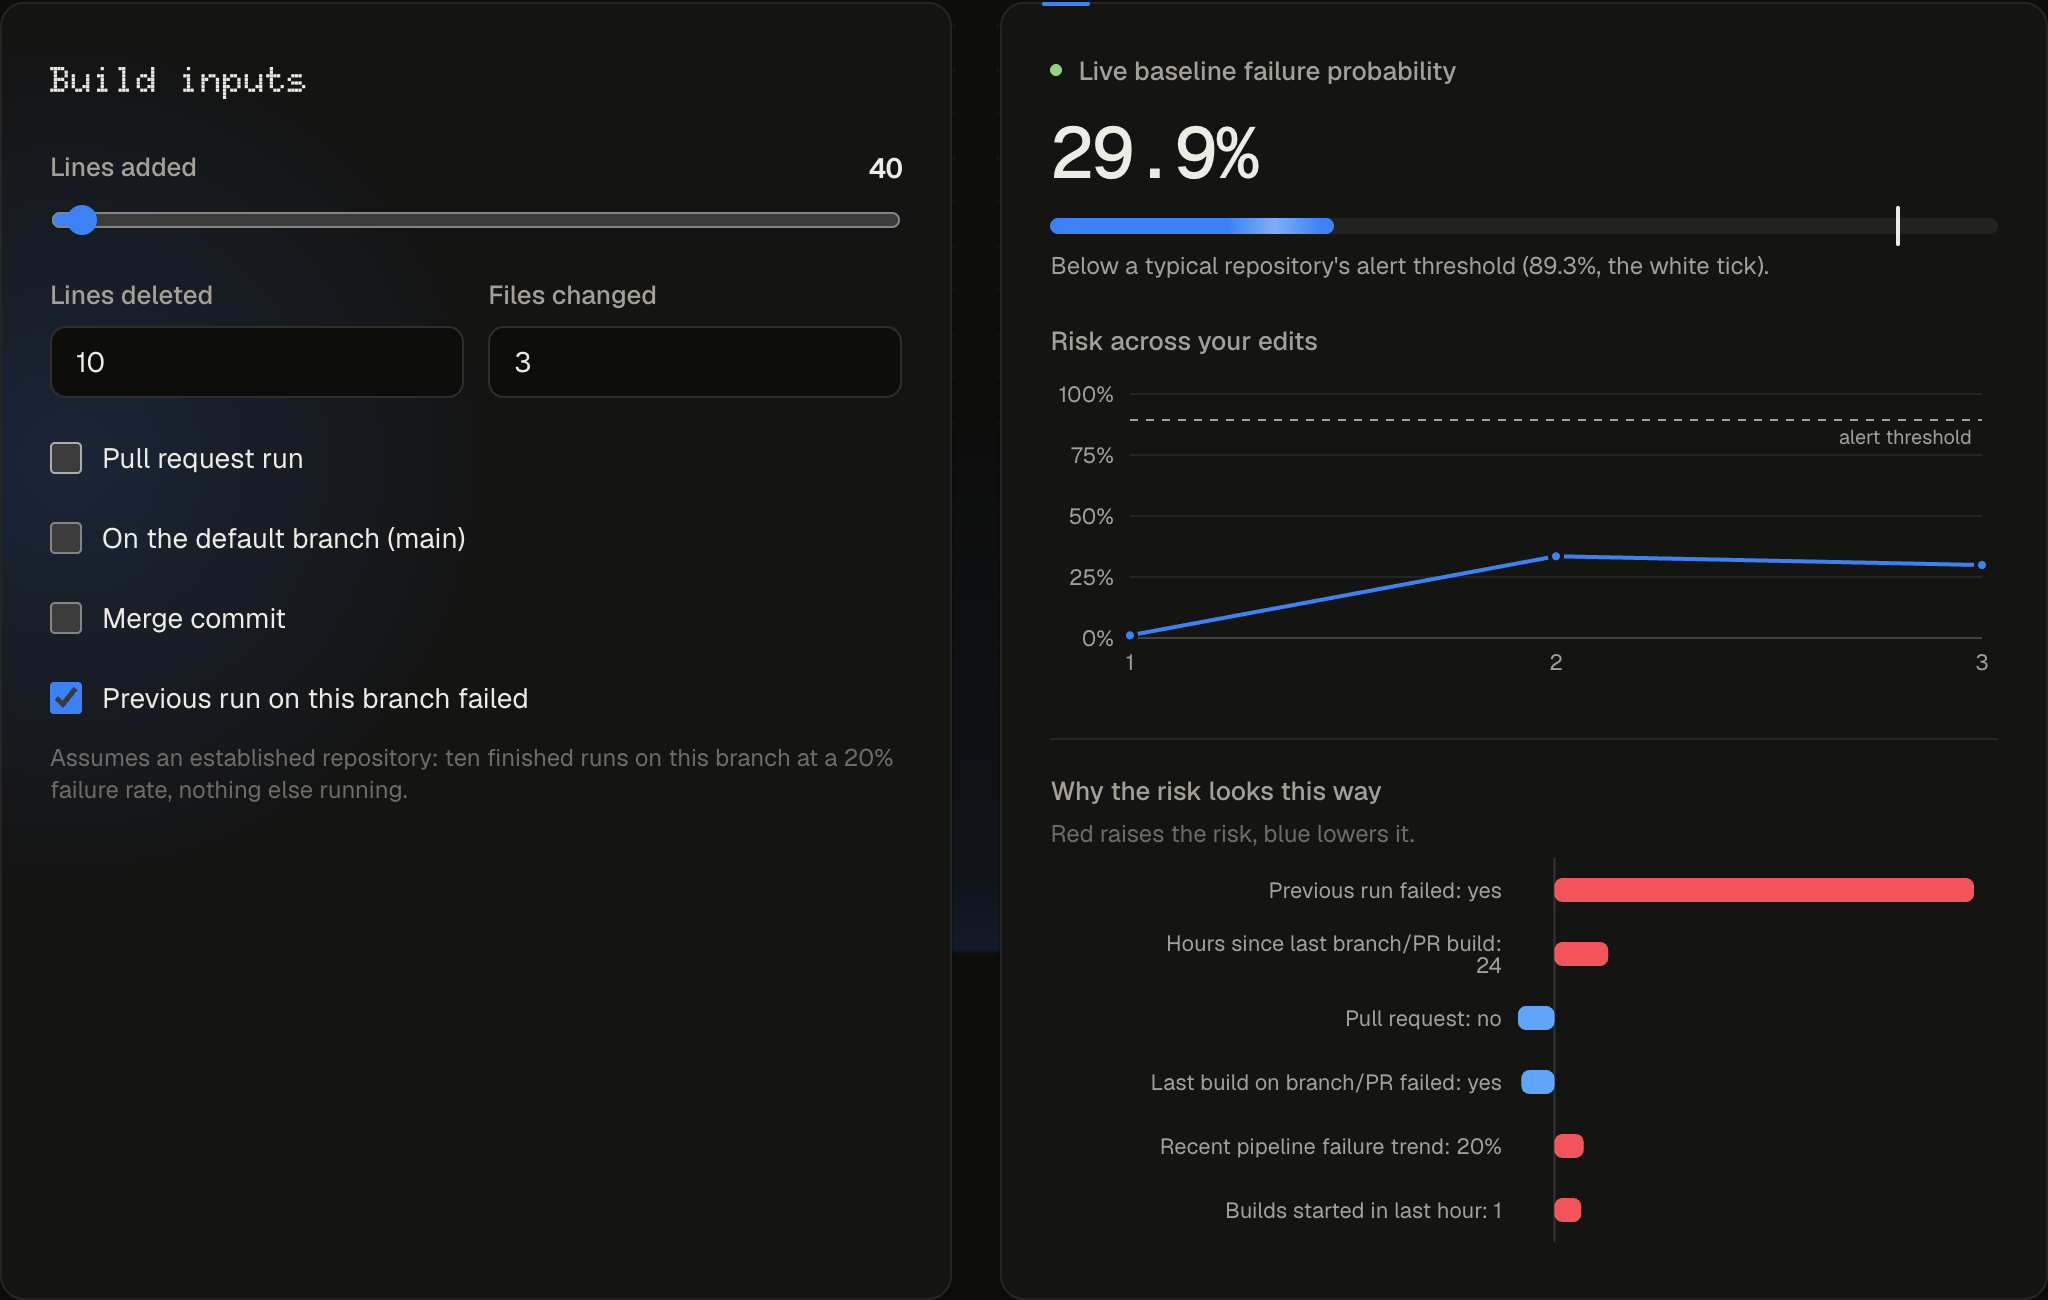
\includegraphics[width=0.9\textwidth]{what_if.png}
\caption{What-If page: whether the previous run of the same workflow failed dominates the explanation}
\label{fig:whatif}
\end{figure}

\section{Testing and Requirement Traceability}
\label{sec:testing}
The project has 84 automated tests, run by GitHub Actions on every pull request together with a production build of the dashboard. They cover:
\begin{itemize}
\item feature engineering, the availability registry and live-versus-training history equivalence;
\item the deployed model and the alert policy;
\item webhook signatures and the requested-to-completed flow, including late deliveries;
\item database migrations, the dashboard endpoints, PDF reports and the read-only demonstration mode.
\end{itemize}
Table~\ref{tab:trace} maps the requirements of Chapter~\ref{ch:srs} to their implementation.

{\renewcommand{\arraystretch}{1.3}
\begin{longtable}{|p{4.4cm}|p{6.2cm}|p{3.2cm}|}
\caption{Requirement-to-implementation traceability}\label{tab:trace}\\
\hline
\textbf{Requirement} & \textbf{Implementation} & \textbf{Verified by}\\ \hline
\endfirsthead
\hline
\textbf{Requirement} & \textbf{Implementation} & \textbf{Verified by}\\ \hline
\endhead
Data collection & TravisTorrent ingestion; GitHub Actions collector; signed webhooks & Webhook and signature tests\\ \hline
Preprocessing & Build collapsing, label rules, availability registry & Preprocessing and registry tests\\ \hline
Feature extraction & Finish-time-safe history, stream and in-flight context & Brute-force and equivalence tests\\ \hline
Failure prediction & \tierE\ model (LightGBM blend); RF, DT, SVM baselines & Model tests; reproduction check\\ \hline
Anomaly / bottleneck detection & Job timing vs.\ history; Isolation Forest & Bottleneck and anomaly tests\\ \hline
Root cause analysis & TF-IDF + k-means; rule-based log diagnosis & Clustering and log-analysis tests\\ \hline
Optimization suggestions & Category-to-suggestion rules; what-if simulation & Suggestion and simulator tests\\ \hline
Dashboard & React dashboard with charts, reports and alerts & Endpoint tests; production build\\ \hline
\end{longtable}}
